%  LaTeX support: latex@mdpi.com 
%  For support, please attach all files needed for compiling as well as the log file, and specify your operating system, LaTeX version, and LaTeX editor.

%=================================================================
\documentclass[entropy,article,submit,moreauthors,pdftex]{Definitions/mdpi} 

% For posting an early version of this manuscript as a preprint, you may use "preprints" as the journal and change "submit" to "accept". The document class line would be, e.g., \documentclass[preprints,article,accept,moreauthors,pdftex]{mdpi}. This is especially recommended for submission to arXiv, where line numbers should be removed before posting. For preprints.org, the editorial staff will make this change immediately prior to posting.

%--------------------
% Class Options:
%--------------------
%----------
% journal
%----------
% Choose between the following MDPI journals:
% acoustics, actuators, addictions, admsci, adolescents, aerospace, agriculture, agriengineering, agronomy, ai, algorithms, allergies, analytica, animals, antibiotics, antibodies, antioxidants, appliedchem, applmech, applmicrobiol, applnano, applsci, arts, asi, atmosphere, atoms, audiolres, automation, axioms, batteries, bdcc, behavsci, beverages, biochem, bioengineering, biologics, biology, biomechanics, biomedicines, biomedinformatics, biomimetics, biomolecules, biophysica, biosensors, biotech, birds, bloods, brainsci, buildings, businesses, cancers, carbon, cardiogenetics, catalysts, cells, ceramics, challenges, chemengineering, chemistry, chemosensors, chemproc, children, civileng, cleantechnol, climate, clinpract, clockssleep, cmd, coatings, colloids, compounds, computation, computers, condensedmatter, conservation, constrmater, cosmetics, crops, cryptography, crystals, curroncol, cyber, dairy, data, dentistry, dermato, dermatopathology, designs, diabetology, diagnostics, digital, disabilities, diseases, diversity, dna, drones, dynamics, earth, ebj, ecologies, econometrics, economies, education, ejihpe, electricity, electrochem, electronicmat, electronics, encyclopedia, endocrines, energies, eng, engproc, entropy, environments, environsciproc, epidemiologia, epigenomes, fermentation, fibers, fire, fishes, fluids, foods, forecasting, forensicsci, forests, fractalfract, fuels, futureinternet, futuretransp, futurepharmacol, futurephys, galaxies, games, gases, gastroent, gastrointestdisord, gels, genealogy, genes, geographies, geohazards, geomatics, geosciences, geotechnics, geriatrics, hazardousmatters, healthcare, hearts, hemato, heritage, highthroughput, histories, horticulturae, humanities, hydrogen, hydrology, hygiene, idr, ijerph, ijfs, ijgi, ijms, ijns, ijtm, ijtpp, immuno, informatics, information, infrastructures, inorganics, insects, instruments, inventions, iot, j, jcdd, jcm, jcp, jcs, jdb, jfb, jfmk, jimaging, jintelligence, jlpea, jmmp, jmp, jmse, jne, jnt, jof, joitmc, jor, journalmedia, jox, jpm, jrfm, jsan, jtaer, jzbg, kidney, land, languages, laws, life, liquids, literature, livers, logistics, lubricants, machines, macromol, magnetism, magnetochemistry, make, marinedrugs, materials, materproc, mathematics, mca, measurements, medicina, medicines, medsci, membranes, metabolites, metals, metrology, micro, microarrays, microbiolres, micromachines, microorganisms, minerals, mining, modelling, molbank, molecules, mps, mti, nanoenergyadv, nanomanufacturing, nanomaterials, ncrna, network, neuroglia, neurolint, neurosci, nitrogen, notspecified, nri, nursrep, nutrients, obesities, oceans, ohbm, onco, oncopathology, optics, oral, organics, osteology, oxygen, parasites, parasitologia, particles, pathogens, pathophysiology, pediatrrep, pharmaceuticals, pharmaceutics, pharmacy, philosophies, photochem, photonics, physchem, physics, physiolsci, plants, plasma, pollutants, polymers, polysaccharides, proceedings, processes, prosthesis, proteomes, psych, psychiatryint, publications, quantumrep, quaternary, qubs, radiation, reactions, recycling, regeneration, religions, remotesensing, reports, reprodmed, resources, risks, robotics, safety, sci, scipharm, sensors, separations, sexes, signals, sinusitis, smartcities, sna, societies, socsci, soilsystems, solids, sports, standards, stats, stresses, surfaces, surgeries, suschem, sustainability, symmetry, systems, taxonomy, technologies, telecom, textiles, thermo, tourismhosp, toxics, toxins, transplantology, traumas, tropicalmed, universe, urbansci, uro, vaccines, vehicles, vetsci, vibration, viruses, vision, water, wevj, women, world 

%---------
% article
%---------
% The default type of manuscript is "article", but can be replaced by: 
% abstract, addendum, article, book, bookreview, briefreport, casereport, comment, commentary, communication, conferenceproceedings, correction, conferencereport, entry, expressionofconcern, extendedabstract, datadescriptor, editorial, essay, erratum, hypothesis, interestingimage, obituary, opinion, projectreport, reply, retraction, review, perspective, protocol, shortnote, studyprotocol, systematicreview, supfile, technicalnote, viewpoint, guidelines, registeredreport, tutorial
% supfile = supplementary materials

%----------
% submit
%----------
% The class option "submit" will be changed to "accept" by the Editorial Office when the paper is accepted. This will only make changes to the frontpage (e.g., the logo of the journal will get visible), the headings, and the copyright information. Also, line numbering will be removed. Journal info and pagination for accepted papers will also be assigned by the Editorial Office.

%------------------
% moreauthors
%------------------
% If there is only one author the class option oneauthor should be used. Otherwise use the class option moreauthors.

%---------
% pdftex
%---------
% The option pdftex is for use with pdfLaTeX. If eps figures are used, remove the option pdftex and use LaTeX and dvi2pdf.

%=================================================================
% MDPI internal commands
\firstpage{1} 
\makeatletter 
\setcounter{page}{\@firstpage} 
\makeatother
\pubvolume{1}
\issuenum{1}
\articlenumber{0}
%\doinum{}
\pubyear{2021}
\copyrightyear{2021}
%\externaleditor{Academic Editor: Firstname Lastname} % For journal Automation, please change Academic Editor to "Communicated by"
\datereceived{} 
\dateaccepted{} 
\datepublished{} 
\hreflink{https://doi.org/} % If needed use \linebreak
%------------------------------------------------------------------
% The following line should be uncommented if the LaTeX file is uploaded to arXiv.org
%\pdfoutput=1

%=================================================================
% Add packages and commands here. The following packages are loaded in our class file: fontenc, inputenc, calc, indentfirst, fancyhdr, graphicx, epstopdf, lastpage, ifthen, lineno, float, amsmath, setspace, enumitem, mathpazo, booktabs, titlesec, etoolbox, tabto, xcolor, soul, multirow, microtype, tikz, totcount, changepage, paracol, attrib, upgreek, cleveref, amsthm, hyphenat, natbib, hyperref, footmisc, url, geometry, newfloat, caption
\usepackage{algorithm2e}

%=================================================================
%% Please use the following mathematics environments: Theorem, Lemma, Corollary, Proposition, Characterization, Property, Problem, Example, ExamplesandDefinitions, Hypothesis, Remark, Definition, Notation, Assumption
%% For proofs, please use the proof environment (the amsthm package is loaded by the MDPI class).

%=================================================================
% Full title of the paper (Capitalized)
\Title{What should I notice? Evaluating the memorability of events for abductive inference.
}

% MDPI internal command: Title for citation in the left column
\TitleCitation{What should I notice?}

% Author Orchid ID: enter ID or remove command
\newcommand{\orcidauthorA}{0000-0000-0000-000X} % Add \orcidA{} behind the author's name
%\newcommand{\orcidauthorB}{0000-0000-0000-000X} % Add \orcidB{} behind the author's name

% Authors, for the paper (add full first names)
\Author{Étienne Houzé $^{1,2}$*, Jean-Louis Dessalles $^{2}$, Ada Diaconescu$^{2}$ and David Menga $^{1}$}

% MDPI internal command: Authors, for metadata in PDF
\AuthorNames{Firstname Lastname, Firstname Lastname and Firstname Lastname}

% MDPI internal command: Authors, for citation in the left column
\AuthorCitation{Lastname, F.; Lastname, F.; Lastname, F.}
% If this is a Chicago style journal: Lastname, Firstname, Firstname Lastname, and Firstname Lastname.

% Affiliations / Addresses (Add [1] after \address if there is only one affiliation.)
\address{%
$^{1}$ \quad EDF R\&D ; \{first\}.\{last\}@edf.fr;
7 boulevard Gaspard Monge, 91120 Palaiseau, France\\
$^{2}$ \quad Télécom Paris; \{first\}.\{last\}@telecom-paris.fr;
19 place Marguerite Perey, 91120 Palaiseau, France}

% Contact information of the corresponding author
\corres{Correspondence: etienne.houze@telecom-paris.fr}

% Current address and/or shared authorship
% \firstnote{Current address: Affiliation 3} 
% \secondnote{These authors contributed equally to this work.}
% The commands \thirdnote{} till \eighthnote{} are available for further notes

%\simplesumm{} % Simple summary

%\conference{} % An extended version of a conference paper

% Abstract (Do not insert blank lines, i.e. \\) 
\abstract{ When confronted with an unprecedented situation, humans typically show good
performance in quickly identifying noticeable past events and proposing them
as possible causal hypotheses. This kind of abductive inference is widely
overlooked in modern AI approaches which rely on massive datasets to learn
associative patterns. Our proposal is to formalize and compute a ``memorability''
score over a set of events recorded from a cyber-physical system.
This score can then be used to select relevant information to be
remembered and to propose causal hypotheses in unusual situations on demand.
The approach is meant to be complementary to more traditional
learning-focused abduction techniques. We provide a theoretical framework based on Algorithmic Information Theory to define the notion of memorability of events. Then, we implement our approaches in two examples based on smart-home scenario to validate our approach in toy cases and illustrate how it could be applied.}

% Keywords
\keyword{Kolmogorov Complexity; Algorithmic Information Theory; Simplicity; Abduction; Surprise} 

% The fields PACS, MSC, and JEL may be left empty or commented out if not applicable
%\PACS{J0101}
%\MSC{}
%\JEL{}

%%%%%%%%%%%%%%%%%%%%%%%%%%%%%%%%%%%%%%%%%%
% Only for the journal Diversity
%\LSID{\url{http://}}

%%%%%%%%%%%%%%%%%%%%%%%%%%%%%%%%%%%%%%%%%%
% Only for the journal Applied Sciences:
%\featuredapplication{Authors are encouraged to provide a concise description of the specific application or a potential application of the work. This section is not mandatory.}
%%%%%%%%%%%%%%%%%%%%%%%%%%%%%%%%%%%%%%%%%%

%%%%%%%%%%%%%%%%%%%%%%%%%%%%%%%%%%%%%%%%%%
% Only for the journal Data:
%\dataset{DOI number or link to the deposited data set in cases where the data set is published or set to be published separately. If the data set is submitted and will be published as a supplement to this paper in the journal Data, this field will be filled by the editors of the journal. In this case, please make sure to submit the data set as a supplement when entering your manuscript into our manuscript editorial system.}

%\datasetlicense{license under which the data set is made available (CC0, CC-BY, CC-BY-SA, CC-BY-NC, etc.)}

%%%%%%%%%%%%%%%%%%%%%%%%%%%%%%%%%%%%%%%%%%
% Only for the journal Toxins
%\keycontribution{The breakthroughs or highlights of the manuscript. Authors can write one or two sentences to describe the most important part of the paper.}

%%%%%%%%%%%%%%%%%%%%%%%%%%%%%%%%%%%%%%%%%%
% Only for the journal Encyclopedia
%\encyclopediadef{Instead of the abstract}
%\entrylink{The Link to this entry published on the encyclopedia platform.}
%%%%%%%%%%%%%%%%%%%%%%%%%%%%%%%%%%%%%%%%%%
\begin{document}
%%%%%%%%%%%%%%%%%%%%%%%%%%%%%%%%%%%%%%%%%%
%The order of the section titles is: Introduction, Materials and Methods, Results, Discussion, Conclusions for these journals: aerospace,algorithms,antibodies,antioxidants,atmosphere,axioms,biomedicines,carbon,crystals,designs,diagnostics,environments,fermentation,fluids,forests,fractalfract,informatics,information,inventions,jfmk,jrfm,lubricants,neonatalscreening,neuroglia,particles,pharmaceutics,polymers,processes,technologies,viruses,vision

\section{Introduction}


As a user has just switch on the TV in her all-equipped living-room, the
lights dim and the window blinds go down. Intrigued by this behavior, she
quickly infers that both light dimming and blind closing occurred as a
consequence of the TV being turned on. How did she come to this conclusion?
By performing \emph{abductive inference} \cite{magnani_abduction_2011}. This mental operation
is a key element of humans' ability to understand the world: from the
observed consequences, they infer the possible causes.
% TODO: answer in the next paragraph?

In this example, there are mainly three possibilities to come to the
conclusion. (1) If the user knows how the smart living-room system works, if she
knows the underlying rules or parameters, she may use this causal
knowledge to perform abduction. (2) If she has no knowledge
about the system but made several observation of the same behavior, she may examine past
correlations and figure out that turning on the TV set often leads the blinds to
close and the lights to dim. (3) If there are no previous occurrences of the event (e.g. it is the first time she turns on the TV
in the living-room), she may still be able to
suspect that the TV is a possible cause for the observed event, just because it appears to her as a memorable recent event (as it is its first occurrence). This example
suggests that human beings are able to use distinct methods to perform abductive tasks
and infer new knowledge, depending on the situation. While the first two mechanisms can be
automated using knowledge bases and statistical methods,the third approach, which can be used without any knowledge of the occurring phenomenon or past occurrences. Instead, it relies on the observation that some events appear more ``memorable'' than others and, as such, can be considered as possible hypotheses if need be.


Defining a score of memorability is not straightforward. First, events can be of different nature, and not directly
comparable. Even for restricted systems such as smart homes, noticeable events
range from device removal to presence detection or unusually high
temperatures. Even for comparable events, the problem is to weigh different characteristics: is a record-high temperature 47 days
ago more memorable than the small deviation recorded just 3 minutes ago? To
our knowledge, no current system proposes to combine various
event types from different devices to compute a unified metrics of
``memorability''. 
% ! Addiction of the follwoing sentence, to show what we can use memorability for.
In addition to the aforementionned use for abductive inference, having access to a computation of memorability would allow a system to summarize a situation to its user by presenting only the most memorable events: for instance, a summary of notable events that occurred during the home owner's absence.

% ? What to do with the "intuition" thing? Keep it? Leave it?
To address this issue, we started from the following intuition: while all
events, regardless of their characteristics or nature, can be uniquely
described using a combination of quantitative or qualitative qualifiers, the most memorable ones are
likely to require less words to be described. ``Last year's hottest day'' is simpler than ``the 182\textsuperscript{nd} day 7 years ago''. How can we quantify this relative simplicity? We could evaluate the complexity of each
description, taking into account both the complexity of the concept words (a date
of occurrence, a temperature ranking), and of the arguments (1st hottest,
182 and 7). The resulting values define the  \emph{description complexity}
of events. Our intuition is that memorable events require simpler and less numerous qualifiers to be
unambiguously described than unremarkable ones.
% ? Response to Ada's remark: added a thing in the 1st paragraph to show what we want ot do with the memorable events.

For machines to implement and compute description complexity, we need a formal framework and computation methods that are in line with human intuition.  Algorithmic Information Theory (AIT) appears to be such a framework, as it is consistent with the human perception of complexity\cite{li_introduction_2008,dessalles2011coincidences,delahaye_numerical_2012}. Our method is as follows: we
consider events as being elements stored in what we call \emph{base memory}. To
reproduce the language features applicable to events, we use \emph
{predicates}, i.e. functions assigning a boolean value to events. For instance, the predicate $\mathtt{date}
(\cdot, 1\_year)$ is \emph{true} of events that occurred last year. Selecting
%%%%%%%%%%%%%%%%%%%%%% ! MOVED FIGURE HERE %%%%%%%%%%%%%%%%%%%%%%%%%%%%%%
\begin{figure}[hb]
    \centering
    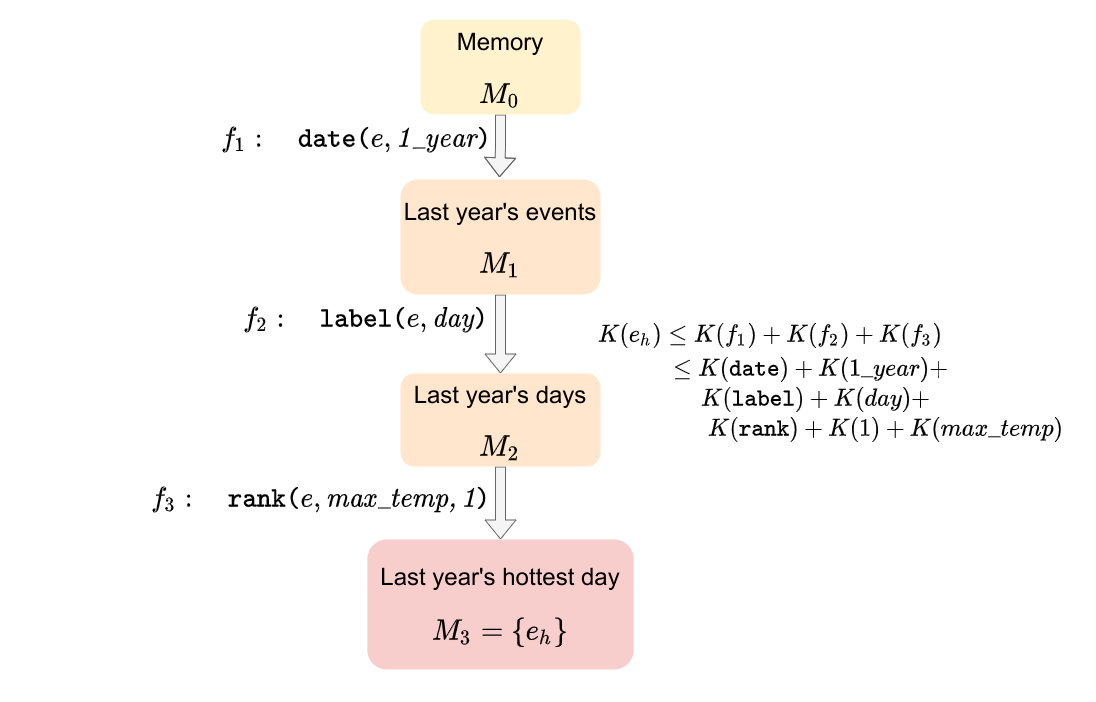
\includegraphics[width=.95\linewidth]{figures/filters}
    \caption{Retrieving an event through successive predicative
        filters. From the base memory (yellow), successive filters select events satisfying the associated predicate (gray arrows). For example,
        filter $f_1$ selects events from last year, i.e. which satisfy the
        predicate $\mathtt{date}(event, 1\_year)$. In this case, successively
        applying filters $f_1$, $f_2$ and $f_3$ yields a unique event $e_h$, last
        year's hottest day. The complexity of this event can then be upper-bounded
        by the complexity of the three filters as they give an unambiguous way
        to describe the event within the memory.}
    \label{fig:filters}
\end{figure}
%%%%%%%%%%%%%%%%%%%%%%! FIGURE END %%%%%%%%%%%%%%%%%%%%%%%%%%%%
all events, from the memory, that satisfy a given predicate corresponds to
a \emph{filter} operation. It generates another memory that is a subset of the previous one.
The filtering operation can then be repeated, selecting
fewer events at each iteration, until a singleton memory is reached. This means that the sequence
of predicates could unambiguously \emph{retrieve} the unique remaining event.
The description complexity of this event can thus be upper-bounded by the
number of bits required to describe the filters used in the retrieval
process. Figure \ref{fig:filters} illustrates this process for the event: ``last year's hottest day''.


% * Paragraph re-written
We will first briefly introduce
some basic notions of Algorithmic Information Theory in subsection~\ref{sec:theory}. We then expose our contribution by presenting in subsection~\ref{sec:computing} our formal definition of memorability and related notions. Then, we present an implementation example of these definitions with two smart-home examples in section~\ref{sec:results}. The results of these experiments are then presented and discussed. Finally we explore other related works in subsection \ref{sec:related} and explore possible extensions of our work in subsection \ref{sec:future}.


% Then, in
% subsection~\ref{sec:computing}, we show how we compute the
% memorability of past events. We illustrate our approach in section~\ref{sec:example} by describing an implementation
% in a smart home simulation context. In section~\ref{sec:related} we review
% a few studies that use complexity theory to generate explanations for the smart home
% and we discuss how our work can be linked with them. We explore potential
% extensions of our work in section \ref{sec:future}

%%%%%%%%%%%%%%%%%%%%%%%%%%%%%%%%%%%%%%%%%%
\section{Materials and Methods}

\subsection{Theoretical Background}
\label{sec:theory}
Kolmogorov complexity formally quantifies the amount of information required
for the computation of a finite binary string\footnote{Though the definition
    holds for some infinite binary strings (think of the representation of the
    decimals of $\pi$), we restrict ourselves here to finite strings.} (or
any object represented by a finite binary
string)\cite{kolmogorov_three_1965,li_introduction_2008}. The complexity $K(s)$ of a (finite) binary string is the length in bits $L(p)$ of the shortest program $p$
which, if given as input to a universal Turing Machine $U$, outputs $s$.

\begin{equation}
    \label{eq:kolmo_def}
    K_{U}(s) = \min_{p}\left\{L(p)|U(p)=s\right\}
\end{equation}

The first notable property of this definition is its universality: while the
choice of the Turing machine $U$ used for the computations appears in the
definition of Equation \ref{eq:kolmo_def}, all results hold, up to an additional
constant, if we change the machine. Think how any Turing-complete programming language can
be turned into any other language, using an interpreter or a compiler program. Since any
Turing machine $U'$ can be emulated by $U$ from a
finite program $p_{U}$, we have the following inequality:

\begin{equation}
    \label{eq:inequality_univ}
    K_{U'}(s) \le l(p_{u}) + K_{U}(s)
\end{equation}

From this first result, we can then define complexity $K(s)$, based on the choice of a reference Turing machine, such that, for any other
machine $U$ taken from the set $\text{TM}$ of Turing machines:

\begin{equation}
    \forall U\in\text{TM}, \forall s, |K(s) - K_{u}(s)| \le C_{U}
\end{equation}

where the additional constant $C_{U}$ does not depend on $s$.

Note that the notion of Kolmogorov complexity involves no requirement on the execution time of
programs, only their length in bits matters for the computation of
complexity. Though Kolmogorov complexity can be shown to be
incomputable\cite{li_introduction_2008},
it can be approximated with
upper bounds by exhibiting a program outputting $s$.

Interestingly, Kolmogorov complexity matches the intuitive
notion and perception of complexity from a human standpoint. For instance, the
complexity of short binary strings evaluated in \cite{delahaye_numerical_2012}
shows similar results to human perception of complex strings and patterns. More
recently, \cite{murena_solving_2020} used Kolmogorov complexity to solve
analogies and showed results close to human expectations.

The bridge between Algorithmic Information Theory (AIT) and human perception of
complexity can be pushed farther thanks to the notions of simplicity and unexpectedness,
which are sometimes regarded of uttermost importance in cognitive science\cite
{chater_simplicity_2003}.
\cite{dessalles2011coincidences} proposes a formal definition of the
unexpectedness $U(e)$ of an event, as the difference between an a-priori
expected causal complexity $K_{w}(e)$ and the actual observed complexity $K
    (e)$.

\begin{equation}
    \label{eq:unexpected} \textit{Unex}(e) = K_{w}(e) - K(e)
\end{equation}

This result comes from the understanding that, while Kolmogorov complexity is
ideally computed using a Turing machine, it can be used as a proxy for modeling
information processing in the human brain, and thus can be used to define a notion of
simplicity or complexity of events.

Definition \ref{eq:unexpected} allows to model phenomena
such as coincidences: imagine that you happen to run into someone in a park.
If this person has no particular link to you, the event will be quite
trivial: the complexity of describing this person will be equivalent to
distinguishing it from the global population, which is also roughly
equivalent to the (causal) complexity of describing the circumstances having brought this person to be in
that park as the same time as you. On the other hand, if you run into your best friend in
a park, as the complexity of describing your best friend is significantly
lower, the description complexity $K(e)$ drops while the causal complexity
$K_W (e)$ remains unchanged. This is why this latter  event appears unexpected.

As \cite{dessalles2011coincidences} suggests a link between the unexpectedness and cognitive relevance, we propose to define the memorability of an event in a similar way.  
Hence, we define the memorability $M(e)$ of an event as the absolute difference between its description complexity $K_d(e)$ and its expected description complexity $K_{exp}(e)$:

\begin{equation}
    \label{eq:memorability}
    M(e) = |K_{exp}(e) - K_d(e)|
\end{equation}

% ? Peut-être ajouter un paragraphe sur pourquoi ne pas directement utiliser la notion de unexpectedness. 1) pas calculable. 2) pas forcément bien définie dans un cas pratique d'application (comment définit la complexité causale ???)
Contrary to the definition of unexpectedness from Equation \ref{eq:unexpected}, we use an absolute value: we do so to acknowledge the fact that events more complex than expected can be memorable as well\footnote{In the original paper \cite{dessalles2011coincidences}, exceptionally complex events are described by considering complexity itself as a way to describe the event: see ``the Pisa Tower effect''\cite{dessalles_pisa_nodate}}. In the next section, we define computational approximations for the description complexity $K_d$ and the expected complexity $K_{exp}$ of events.

\subsection{Computing the memorability of events}
\label{sec:computing}
\subsubsection{Retrieving an event}

%Computing the memorability of events begins with the introduction of formal definitions of events, how they are stored, how we can describe them and how these descriptions can be used to retrieve them.
We define \emph{events} as data points augmented with a \emph{label} indicating their nature (temperature event, failure event, addition/removal of a device) and a timestamp of occurrence. Formally:

\begin{equation}
    \label{eq:event}
    e = (l, t,\mathcal{D})
\end{equation}
% ! response to Ada's remark: there is a hidden unique ID in the implementation, to distinguish between events; however this is not used to retrieve the event, as it is not a defining characteristics.
where $l$ is the label, $t$ the timestamp and $\mathcal{D}$ a vector of properties characterizing $e$: its duration, the maximum temperature reached, the sensor name, its position, etc. Labels can also be considered as classes of events, of which each event is a particular instance.

To model how humans are able to describe events by using qualifiers, we use \emph{predicates}: Boolean functions operating on events and, possibly, additional parameters: $\pi(e, a_1, a_2, \dots, a_n) \mapsto \{O,1\}$ is a predicate of arity $n$ operating on event $e$. In the rest of this paper, we will prefer the equivalent notation $\pi(e, k) \mapsto \{0,1\}$, where $k$ is a binary string encoding the sequence of arguments $a_1, \dots, a_n$. Using this notation, the predicate $\pi$ becomes a boolean function operating on $\mathbf{E} \times \{0,1\}^*$, where $\mathbf{E}$ denotes the set of all events:

\begin{equation}
    \label{eq:predicate}
    \pi : \begin{cases}
        \mathbf{E}\times \{0,1\}^{*} & \mapsto \{0,1\}    \\
        (e, k)                        & \mapsto \pi_{k}(e)
    \end{cases}
\end{equation}

As an example of predicate, consider $\pi = \mathtt{year}$ and $k$ a string encoding the number $1$, thus
constructing the predicate $\mathtt{year(}e, 1\mathtt{)}$, which tells whether
the event $e$ occurred $1$ year ago.

% ! response to Ada's remark: complexity computations don't consider time complexity, only program length. Indeed, using a FILO structure for the memory makes sense implementation-wise, but it does not affect the definitions of complexity and memorability. 
As events occur, they are stored in the  \emph{base memory} $M_0$. As they are not directly comparable, the memory $M_0$ can be considered as having the structure of an unordered set. We denote by $\mathcal{M}$ the set of all subsets of $M_0$. By extension, elements of $\mathcal{M}$, i.e. subsets of $M_0$, are also called \emph{memories}.

By applying a given predicate $\pi$ to all events contained in a memory $M \subseteq M_0$, and selecting only events satisfying $\pi$, one gets another memory $M_1 \subseteq M \subseteq M_0$. We call this operation a \emph{filter}:

\begin{equation}
    \label{eq:filter}
    f_{\pi, k}: \begin{cases}
        \mathcal{M} & \mapsto \mathcal{M}           \\
        M           & \mapsto \{e \in M | \pi_k(e) \}
    \end{cases}
\end{equation}

For instance, using the same $\pi = \mathtt{year}$ and $k=1$ as above, we can
build the filter $f_{\pi, k} = \mathtt{last\_{}year}$, which selects all events
that occurred last year.

As the output of a filter applied to a memory $M$ is another memory
object $M' \subseteq M$, we can compose filter
functions. A sequence of such filters is called a \emph{retrieval path}

\begin{equation}
    \label{eq:ret_def}
    p = (f_{\pi_{1}, k_{1}}, \dots, f_{\pi_{n}, k_{n}})
\end{equation}

By definition
$p(M) = f_{\pi_{n}, k_{n}}(\dots(f_{\pi_{1}, k_{1}}(M)))$.
In case the result of the operation $p(M)$ contains a single element
$e$, we say that the path $p$ \emph{retrieves} the element $e$ from $M$, and write
$p(M) = e$. In the example shown in Figure \ref{fig:filters}, the three filters $f_1, f_2, f_3$ form a retrieval path retrieving the event ``last year's hottest day'' from the base memory $M_0$.

\subsubsection{Description complexity of events}

As presented in sec. \ref{sec:theory}, we are interested in computing an approximation of the description complexity of an event $e$. From the above definitions, if there is a path $p$ retrieving $e$ from the base memory $M_0$, i.e. $p(M_0) = e$, this path provides a possible unambiguous description for $e$. We therefore define the description complexity of $e$ as the minimum complexity of a path $p$ retrieving $e$ from the base memory $M_0$.

\begin{equation}
    \label{eq:k_desc}
    K_d(e) = \min_{p \in P_\infty} \{L(p) | p(M_0) = e\}
\end{equation}

where the bit-length $L(p)$ of a retrieval path is defined as the number of bits of a string encoding the path. If we limit ourselves to prefix-free strings encoding predicates and arguments, the total bit length is given by:

\begin{align}
    \label{eq:bit_lenght_p}
    L(p) & = L((f_{\pi_1,k_1}, \dots, f_{\pi_n, k_n}))     \\
         & = L(\pi_1) + L(k_1) + \dots + L(\pi_n) + L(k_n)
\end{align}
where $L(\pi_\square)$ and $L(k_\square)$ respectively denote the length, in bits, required to express the predicate's concept and program. This length may vary depending of the encoding choice, see Section \ref{sec:results} for an example.

By considering only a finite number of possible predicates $\pi$ and arguments $k$, and a maximum path length, we can construct a finite set $P$ of possible retrieval paths. By limiting the search over this set, we get an upper bound of description complexity, and use this upper bound as an approximation:

\begin{equation}
    \label{eq:approx_k_desc}
    K_d(e) \leq \min_{p \in P \land p(M_0) = e} L(p) = \min_{p \in P \land p(M_0)=e} \sum_{f_{\pi, k} \in p} L(\pi) + L(k)
\end{equation}

\begin{algorithm}
    $\mathtt{current_{explore}} \leftarrow [(\mathcal{M}, 0)]$ \;
    $\mathtt{future_{explore} \leftarrow} [\;]$ \;
    $\mathtt{pass} \leftarrow 0$ \;
    $\mathtt{K(e)} \leftarrow +\infty$ \;
    \While{$\mathtt{current_{explore}} \neq [\;]$ \textbf{and} $\mathtt{pass} < \mathtt{max\_pass}$}{
    \For{$(\mathtt{M_{prev}}, \mathtt{K_{prev}}) \in \mathtt{current_{explore}}$}{
    \For{$\mathtt{\pi \in \mathcal{P}}$}{
    \For{$\mathtt{k \in \{0,1\}^{*}}$}{
    $\mathtt{K_{current} \leftarrow l(\pi) + l(k) + K_{prev}}$ \;
    \If{$\mathtt{K_{current}} > \mathtt{max_{complex}}$}{
        \textbf{break} \;
    }
    $\mathtt{M'} \leftarrow f_{\pi,k}(\mathtt{M_{prev}})$ \;
    \eIf{$\mathtt{M'} = \mathtt{\{e\}}$}{
        $\mathtt{K(e) \leftarrow \min(K(e), K_{current})}$ \;
    }{
        $\mathtt{future_{explore}.append((M', K_{current}))}$\;
    }
    }
    }
    }
    $\mathtt{current_{explore}} \leftarrow \mathtt{future_{explore}}$ \;
    $\mathtt{future_{explore}} \leftarrow [\;]$ \;
    $\texttt{pass} \leftarrow \mathtt{pass} + 1$\;
    }
    \caption{Iterative computation of the approximate complexity}
    \label{alg:complex_iter}
\end{algorithm}

The approximation of description complexity from Equation \ref{eq:approx_k_desc} allows for
a direct implementation, which is shown in Algorithm \ref{alg:complex_iter}. This
algorithm operates iteratively: starting from the base memory $M_0$
(line 1), we apply all possible predicate concepts $\pi$ from a given finite set
$\Pi$ and programs $k$ (lines 6-7), up to a given length $\mathtt
    {max\_len}$ bits, and apply them: $M' = f_{\pi, k}(M)$ (line 12). We then store
the pairs $(M', \mathtt{len(}\pi, k\mathtt{)})$ in an array $\mathtt{future_
            {explore}}$. At the end of the iteration, the results of the filters become the
memories which will be explored during the next iteration(lines 21--23). Each
pass thus explore retrieval paths of increasing length. When a singleton memory
is reached, the complexity of its unique element is upper-bounded with the
length of the corresponding retrieval path (line 14).
% ! response to Ada's comment: yes, this works well ;-) It is even implemented in the code. However, given that time complexity does not impact the definitions of complexity, I decided to present the simplest program, not the most optimized, for the sake of clarity.

\subsubsection{Computing Memorability}
As stated in Equation \ref{eq:memorability}, we define memorability $M(e)$ as the absolute difference between the description complexity of an event and its expected value. As we've just defined $K_d(e)$ and provided an approximation in Equation \ref{eq:approx_k_desc}, we now focus on defining the \emph{expected} description complexity of an event, $K_{exp}(e)$ that appears in Equation \ref{eq:memorability}

$K_{exp}(e)$ evaluates the complexity that the user, or the system, would expect for the occurrence of event $e$ to have, based on their previous knowledge. In our framework, this prior knowledge consists of the base memory $M_0$. The expected complexity of the event $e$ can be computed with a simple first-order approximation, i.e. estimating the average complexity of ``similar events'' over the base memory $M_0$.

Still, there is a difficulty in defining what
should be considered \emph{similar} events. Given that we deal with non comparable events, we may define the notion of similarity by referring once again to \emph{predicates}. For a given event $e$ and a given predicate $\pi_k$, we define a $\pi_k$-neighborhood of $e$ as the set $N_{\pi, k}(e)$ of all other events satisfying $\pi_k$.

\begin{equation}
    \label{eq:similar}
    N_{\pi, k}(e) = \{e'\in M_0, (e' \neq e) \wedge \pi_k(e')\}
\end{equation}

Now, when considering, for all possible predicates $\pi_k$, the corresponding
neighborhoods $N_{\pi, k}(e)$, with the convention that $N_{\pi, k}(e) = \emptyset$
if $e$ does not satisfy $\pi_k$, we can compute an average expected complexity for $e$, by summing the complexity of events in all neighbourhoods of $e$ and dividing the total by the number of events in the neighborhoods:

\begin{equation}
    \label{eq:expected}
    K_{exp}(e) = \frac{
    \sum_{\pi, k} \sum_{e' \in N_{\pi, k}(e)} K_d(e')
    }{
    \sum_{\pi, k} |N_{\pi, k}(e)|
    }
\end{equation}

This definition is consistent with the intuitive idea that more similar events should weigh more in the computation. Indeed, if $e'$
is very similar to $e$, it will appear in many neighborhoods, since it
satisfies most of the predicates that $e$ satisfies. Therefore, it will
be present in more terms in Equation \ref{eq:expected}, and will weigh more in
the final result.
% ! response to Ada's comment: Yes, it is. If a point belongs to many neighbourhoods, with many points in each, it will be hard to distinguish from the other points. So, its expected complexity is hard. Think, for instance, of the expected complexity for a human being: it will be roughly log2(7000000000) bits, for a randomly picked person. If this person is known to you, it will be simpler to describe her. 

\subsubsection{From memorability to abduction}
% TODO : see ada's comment for this part
Abductive inference builds upon the computation
of the memorability score. \emph{Knowing} that we want to find a cause $c$
for an observed effect $e$, we try to find the most remarkable event in past
memory that is related to $e$. While our ``memorability'' score identifies remarkable past events, it does not take into account their relatedness to $e$.

The knowledge attached to the occurrence of $e$ can be integrated into the description complexity definition by using conditional complexity $K_d(c | e)$: The information contained in $e$ is considered as given, and therefore ``free'' in terms of complexity. For instance, when looking for a cause of
an anomaly in the living-room, other anomalies occurring in the same
living-room will be simpler, as the location ``living-room'' is already known
from the observation of the current anomaly.

Formally, we now consider that knowledge of the effect is given. This consists, for instance, of appending a description of effect $e$  is appended to all programs $k$:
$\pi_{k::e}(c)$, where $::$ is the append operation. The set of paths obtained with such predicates is noted $P^\infty_e$. This append operation is free in terms of bit-length in the computation of complexity, since the effect event $e$ is an input of the problem. Therefore, we have $L'(\pi_{k::e}) = L(\pi_k) = L(\pi) + L(k)$. We get a definition for the conditional description complexity:

\begin{align}
    \label{eq:abd_k}
    K_d(c | e) & = \min_{p \in P^\infty_e} \{L'(p), \quad p(M_0)=c \}                                                \\
               & = \min_{p \in P^\infty_e} \left\{\sum_{f_{\pi, k::e} \in p} L(\pi) + L(k), \quad p(M_0) = c\right\}
\end{align}

This new conditional description complexity translates the additional information provided to the
system when answering a user's request. It can then be averaged over similar events to compute the expected conditional description complexity, $K_{exp}(c|e)$. From this, we come to the definition of the conditional memorability, which measures how memorable an event $c$ turns out to be in the context of the occurrence of another event $e$:

\begin{equation}
    \label{eq:cond_mem}
    M(c|e) = |K_{exp}(c|e) - K_d(c|e)|
\end{equation}

Conditional memorability encapsulates the idea
presented as the motivation of this paper: when confronted with a surprising
situation, and in the absence of any other source of information, events that appear more memorable than others, with regards to the target event will be selected as potential causes. As such, our conditional memorability score provides a ranking that can be used for abductive inference.

This metrics answers the different problems exposed in the introduction: by using a universal measure for complexity, bits, it allows to compare values from different dimensions. For instance, it solves the dilemma of recent events: is a big event a long time ago more memorable than a smaller one only a few minutes ago? The answer from conditional memorability is that "it depends". It depends on the complexity cost set for the predicates describing time and the magnitude of the event. These complexity costs should reflect the user's perception of the different dimensions (see Section \ref{sec:future}).


%%%%%%%%%%%%%%%%%%%%%%%%%%%%%%%%%%%%%%%%%%
\section{Results}
\label{sec:results}
\subsection{Setup}

We design two different setups to test our approach. Both are inspired from smart home use cases.  This choice of
configuration is motivated by the challenges posed by smart homes for abductive
inference: i) as the number of connected devices increases, more events are
recorded, making the detection of memorable events more important; ii) smart
homes are prone to experience atypical situations, highly dependent on the context,
for which pre-established relations might fail to find good abduction
candidates. Our choice was also motivated by
the existence of previous work involving smart home simulations capable of quickly generating data from which we could extract events and test our methods.

\subsubsection{Scenario 1}
In this setup, we aim to reproduce the example mentioned in Section \ref{sec:introduction}: the installation of a brand new smart TV causes unpredictable effects on the light of a room.
To play this situation, we created a set of events covering a period of 100 days, corresponding to the past knowledge of the house. Two kinds of events are recorded: ``TV event'', corresponding to TV use, and luminosity events, describing the luminosity of the room at a given time. Low lights occur at night, and can occasionally occur during daytime, with a small probability. On the 100\textsuperscript{th} day, a ``TV event'' is recorded with a different ``device'' characteristic. Shortly after, the light lowers, which is recorded in the following ``light'' event.

\subsubsection{Scenario 2}
We consider an experimental smart home setup, with various sensors, which we simulate over a period of time
To carry out the simulation, we built custom modules into the existing iCasa
smart home simulator\cite{lalanda_self-aware_2017}. ICasa
offers a simulation of autonomic systems that can handle internal communications,
the possible insertion of new components at runtime, or the deletion or modification of existing
components. We used a basic scenario consisting of a house with four rooms,
a single user, and an outdoor zone. All four rooms are equipped
with a temperature controller system that monitors and controls heaters (fig.
\ref{fig:view}).

\begin{figure}[ht]
    \centering
    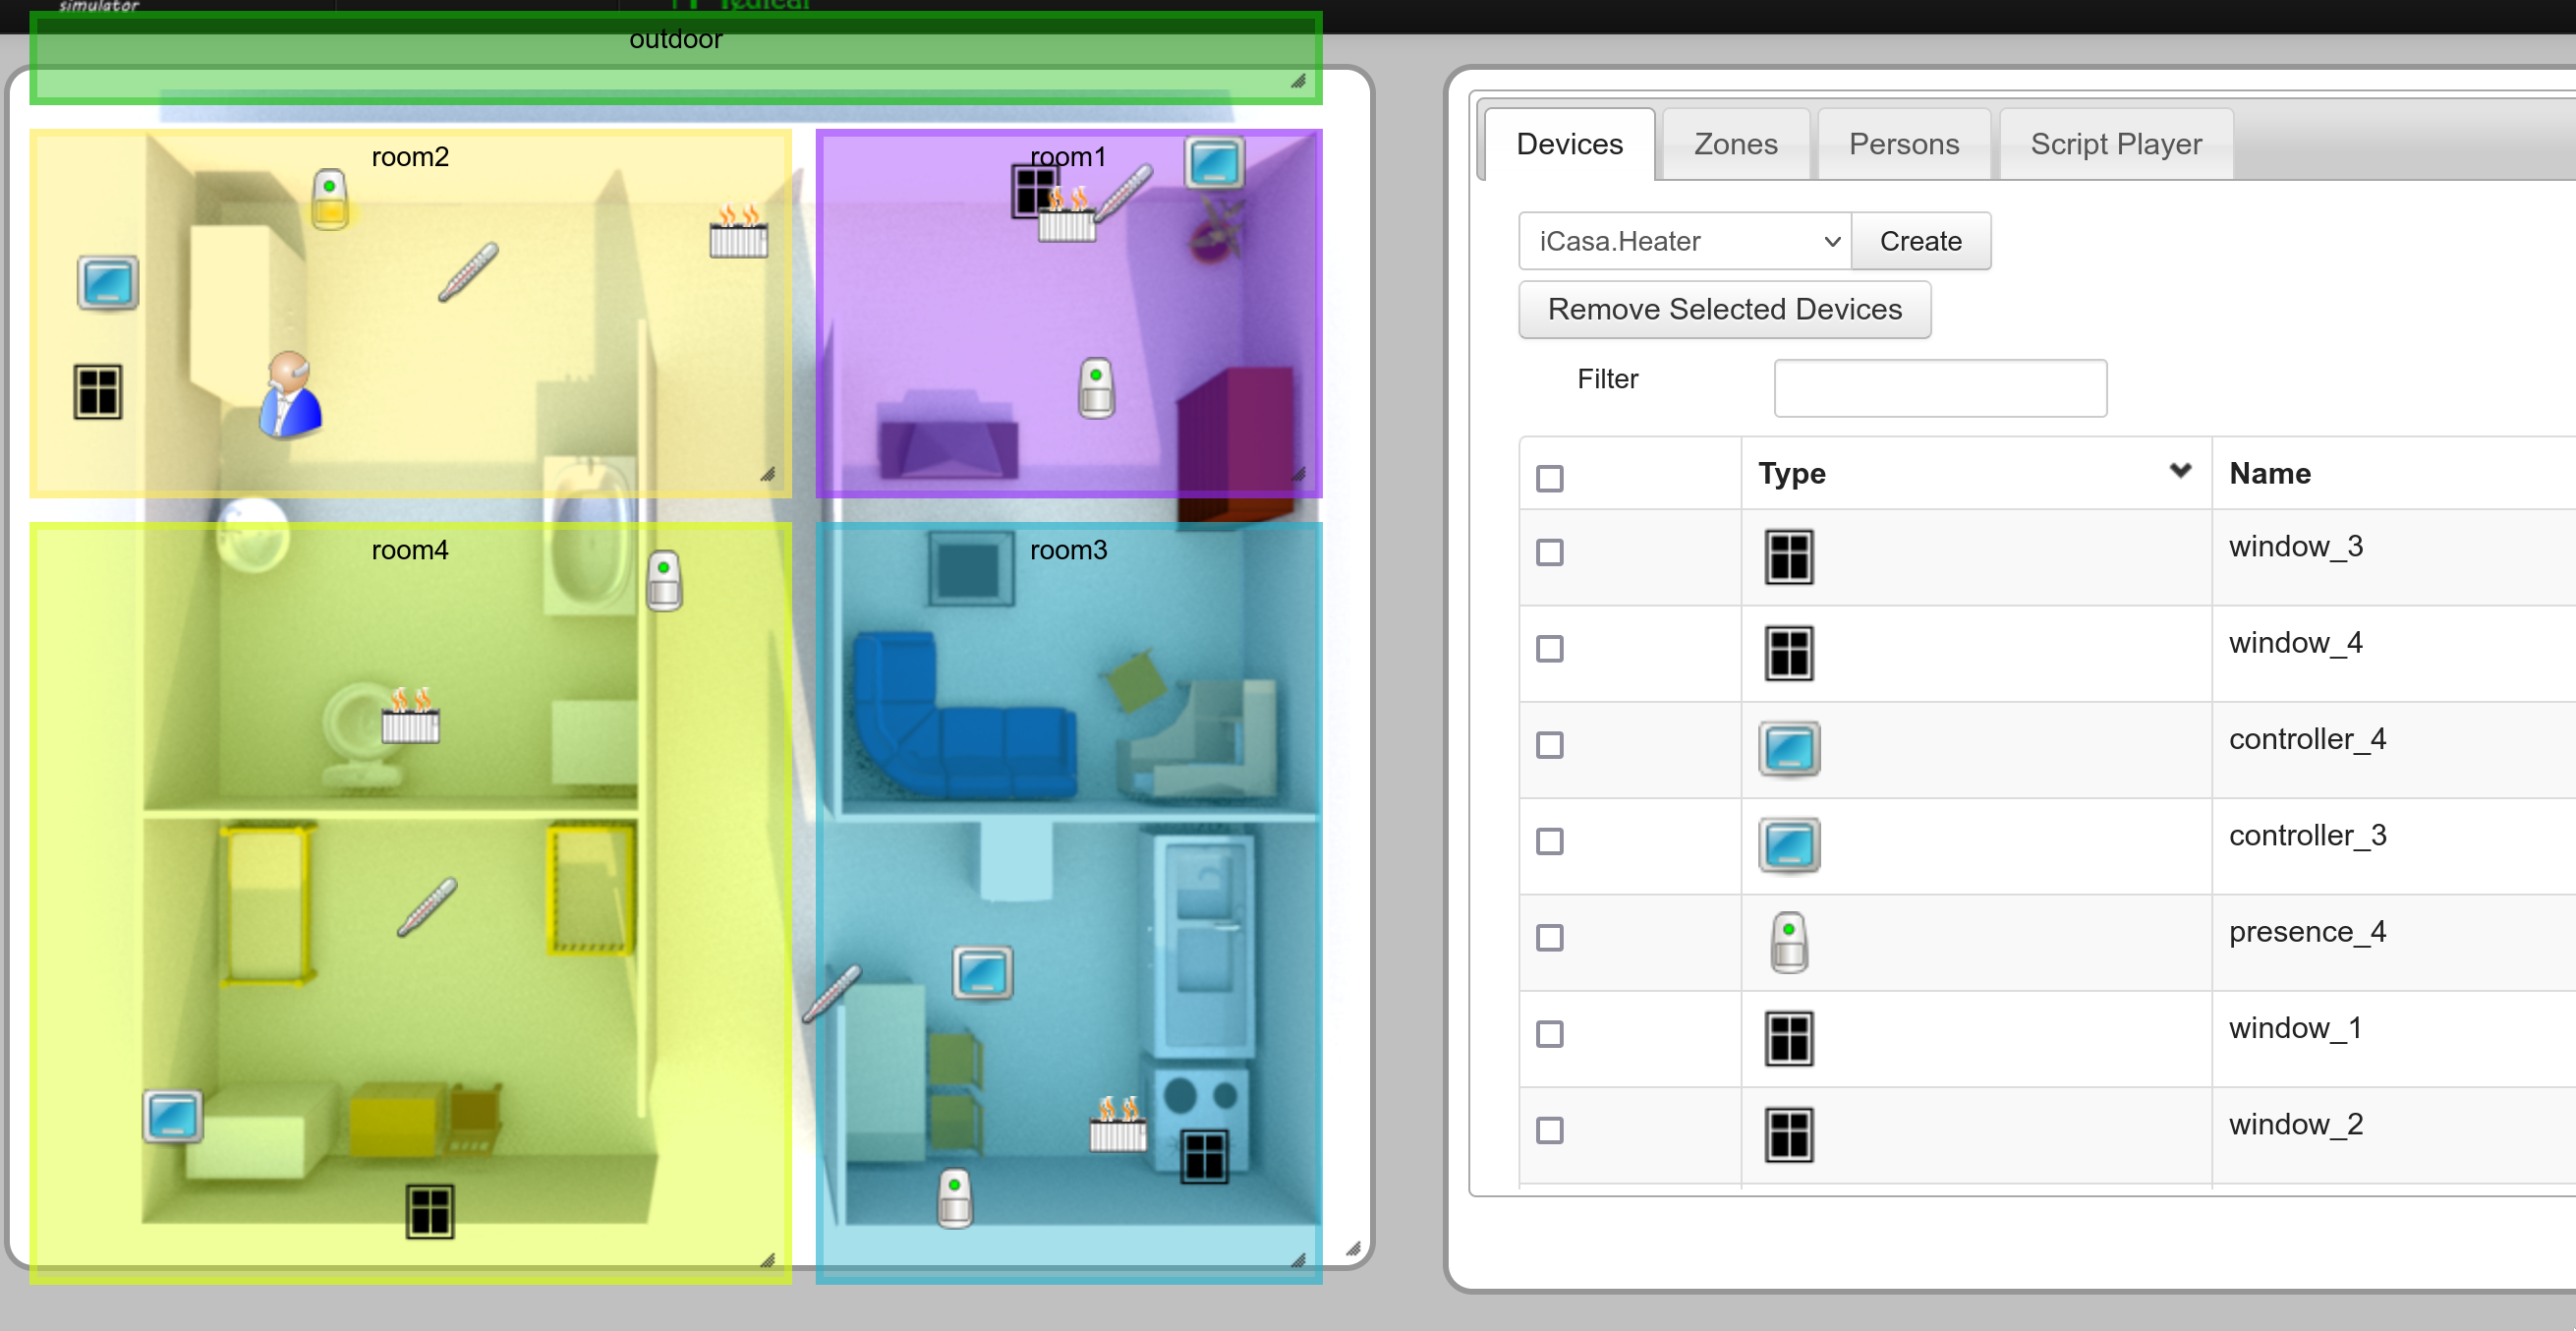
\includegraphics[width=.8\linewidth]{figures/simulator}
    \caption{View of the simulator's web interface provided by iCasa. The four
        rooms are visible, with their equipment and the user.}
    \label{fig:view}
\end{figure}

Based on this, we implemented a scenario spanning over 420 days, and
comprising a daily cycle of outdoor weather (temperature and sunlight) fluctuations, as well
as user's movements. All these daily changes create non-noticeable events,
serving as a background for our experiments. To produce outstanding
events, we randomly generated about twenty events, spanning over the whole
duration of the simulation, of different kinds:

\begin{itemize}
    \item Unusual weather: the outdoor conditions are set to unusually high or
          low temperatures.
    \item Heater failures: heater may break down, making them turn off regardless
          of the command they receive.
          % \item User's absence: the user goes out of the building for an extended
          %       period of time.
    \item Device removal/addition: a device is removed, or another one is added
          to the system.
\end{itemize}


\begin{figure}[ht]
    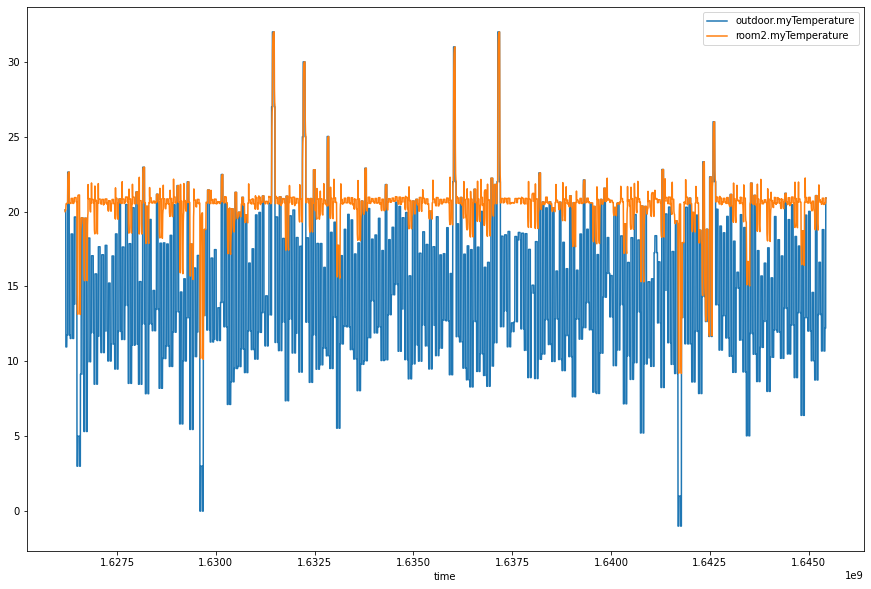
\includegraphics[width=\linewidth]{figures/ts_example}
    \caption{Time series data from the simulation: outdoor temperature (blue) and
        controller temperature of a room (orange). To be used in our framework, these time series data are
        processed by a simple threshold-based event detection.}
    \label{fig:ts_example}
\end{figure}

The values observed from all devices and zones was sampled throughout
the simulation run. The resulting data (figure
\ref{fig:ts_example}) was then used as a basis for our experiments.
We then process the time series data to identify and characterize events.
Since the selection of events is not the focus point of our present work (see sec.
\ref{sec:related}), we perform event detection merely based on threshold and precomputed conditions.


\subsection{Implementing the complexity computation}

We implemented the computation of both the description complexity and the memorability score into a Python object, called the \texttt{SurpriseAbductionModule}. Apart from the base memory of events $M_0$, this module contains a set of predefined predicates $\Pi$ to characterize events. For instance, for scenario 2, the predicates we use are the following:
\begin{itemize}
    \item $\mathtt{label(e, k)}$: whether the event $e$ has the label ranked
          $k^{th}$ in the label list.
    \item $\mathtt{rank(e, r, a)}$: whether the event $e$ has the rank $r$
          along axis $a$.
    \item $\mathtt{day(e, k)}$: whether the event $e$ occurred $k$ days ago.
          % \item $\mathtt{randomChoice(e, k)}$: whether the event $e$ id matches the program $k$, which can be regarded as a random seed.
    \item $\mathtt{month(e, k)}$: whether the event $e$ occured $k$ months ago.
    \item $\mathtt{location(e, k)}$: whether the event $e$ occurred in zone
          $k$.
\end{itemize}

Similar predicates were used for scenario 1, with the notable exception of the addition of a \texttt{RandomPick} predicate, which is true if the id of the event matches a random program seed $k$. Using this predicate and the associated filter in only one of the two illustrative examples shows the importance of allowing random selection in the complexity computation. Furthermore, it could be argued that in some case, random selection of an event is not possible.

The description length $L_{\pi, k}$ of using a predicate is computed as follows: since the set of predicates is finite and known, $L(\pi) = \log2(|\Pi|)$ are enough to describe the predicate concept $\pi$\footnote{This approach gives an equal complexity to all predicate concepts. While this could be argued when using many concepts, as humans do, we deemed better, for our small examples, to consider all concepts as equal.}. To encode the argument $k$ of the predicate, we used the prefix-free Elias delta code\cite{elias_universal_1975}, which requires $L(k) = \log2(k) + 2 \log2(\log2(k)+1) + 1]$ bits. The total cost of describing $\pi_{k}$ therefore is

\begin{equation}
    \L(\pi, k) = \log2(|\Pi|) + \log2(k) + 2 \log2(\log2(k) + 1) + 1
\end{equation}

With a straightforward implementation of memory, predicates and filters, we could run alg. \ref{alg:complex_iter} worked, though, as expected, it took too
long to be usable in realistic scenarios with hundreds or thousands of events to
consider. In order to facilitate and speed up computations, we also implemented
the following improvements:
\begin{itemize}
    \item The memory object was augmented with various built-in rankings, allowing
          for faster operations during future filtering. For instance, since the memory
          object keeps a mapping from timestamp to events one can perform a quick
          filtering by date without having to loop over all stored element. This convenient mapping,
          however, is not directly used to retrieve events by their date of occurrence, so as to
          preserve the theoretical model of memory as an unordered set, as presented in
          section \ref{sec:computing}.


    \item Each of these predicates holds the property that, in addition to
          \texttt{True} and \texttt{False}, they can return another value,
          \texttt{None}, which is theoretically treated as \texttt{False} but carries
          the additional information that this predicate concept will also be false for
          any other element of the memory for any subsequent program $k$. This allows to
          effectively break the innermost loop in alg. \ref{alg:complex_iter}.

    \item Some of the filters, for instance the date and rank filters, were
          hard-written. Events can be selected from these precomputed mappings over the memory objects
          rather than by testing a predicate over all memory elements.
\end{itemize}


\subsection{Results}
\label{sec:example}

\subsubsection{The ``TV'' scenario:}
\paragraph{Memorability}
The computation of the description complexity measure for the 2400 events recorded in this scenario took around 90 seconds using an i7-8600u laptop. The resulting complexities, in Figure \ref{fig:scenar1_complexity}, show that TV events appear more simple than luminosity events. In fact, for most luminosity events, the complexity corresponds to the random choice complexity, 25 bits in this example. This pattern comes from the number of luminosity events per day, 24, is too high to consider the retrieval path $day,  randomPick$ simpler than $randomPick$ from the entire memory, except for the most recent days, which appear simpler (on the right-hand side of Figure \ref{fig:scenar1_complexity})
\begin{figure}
    \centering
    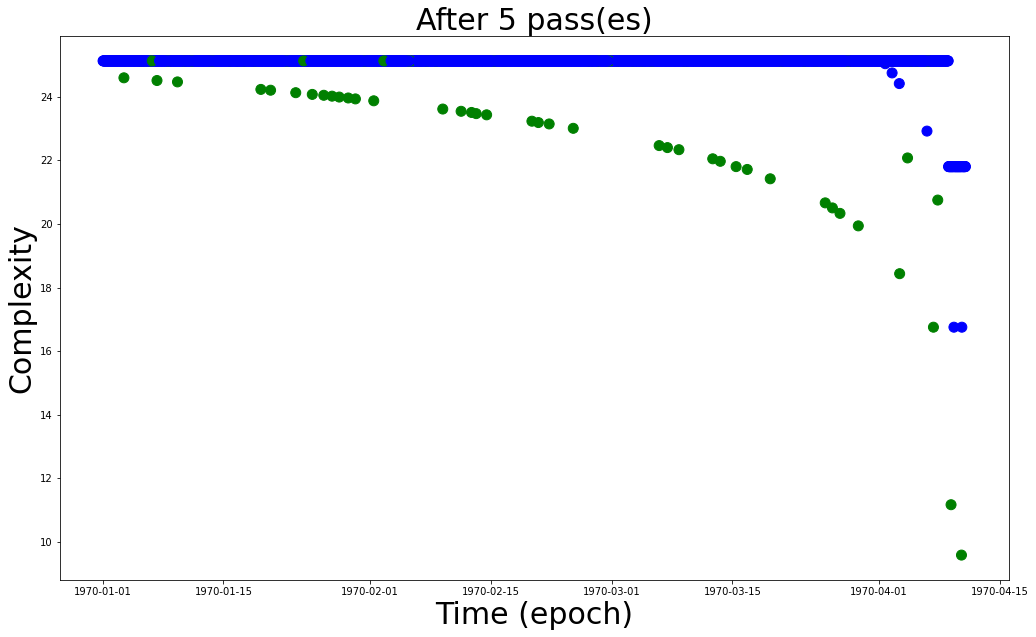
\includegraphics[width=.7\linewidth]{figures/memorability_scenar_1.png}
    \caption{Description complexity for events recorded in the TV scenario. Luminosity events are shown in blue, TV events in green}
    \label{fig:scenar1_complexity}
\end{figure}

\paragraph{Abduction}
To show the potential application to abductive inference, we use our approach to the first scenario, to see if memorability alone can find the brand new TV to be a reasonable cause for the sudden low light.

The result of our algorithm is given in Table \ref{tab:abduction_res}. It shows that the system correctly identifies the TV as being the cause. The reason for this choice is that, since the smart TV's device ID is unique among all other events of type ``TV'', its description complexity is very low.

% \begin{figure}
%     \centering
%     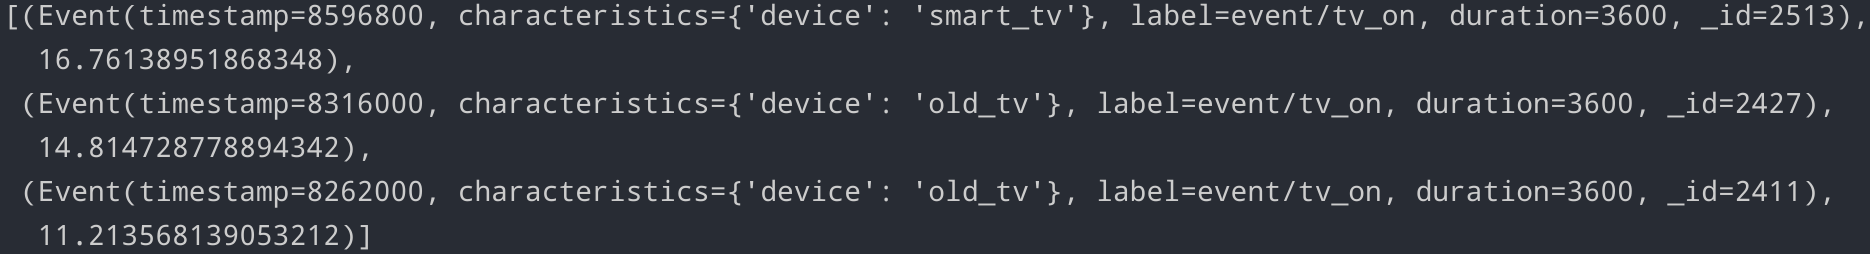
\includegraphics[width=.8\linewidth]{./figures/abduction_1_results}
%     \caption{Outputs of the memorability-based abduction module. This represent the 3 events in the memory having the highest memorability score relative to the consequence event.}
%     \label{fig:abduction_res}
% \end{figure}

\begin{table}
    \centering
    \begin{tabular}{l|c|c}
        Event Id & Description                   & Relative memorability (bits) \\
        \hline
        2513     & Use of smart TV               & 16.76                        \\
        2427     & Last use of the old TV        & 14.81                        \\
        2411     & Second-last use of the old TV & 11.21
    \end{tabular}
    \caption{Output of the memorability-based abduction module: top 3 events for the relative memorability metrics.}
    \label{tab:abduction_res}
\end{table}

\subsubsection{The ``temperature'' scenario:}
% \paragraph{Memorability}

The results of the description complexity evaluation, for the described setup,
are shown in Figure \ref{fig:computed_cplx}. The entire computation, over 4
iterations (meaning that retrieval paths contained at most 4 filters), took
around 30 seconds on a commercial laptop with an i7-8700u CPU.

The general trend appears different from the ``TV example'' presented in Figure \ref{fig:scenar1_complexity} : instead of having a capped complexity score, a logarithmic trend appears. This phenomenon is due to the absence, in this example, of the \texttt{randomPick} predicate; instead, usual events, with outstanding particularity, can be retrieved by using the \texttt{day} predicate and a \texttt{label} predicate. As such, it appears that most days are considered usual by our memorability score, creating the main logarithmic sequence of blue dots: there is no better way to retrieve them than simply giving the day of their occurrence. On the other hand, some events stand out in terms of
complexity: some appear simpler, as they can be distinguished by using their
rank along some axis (``the hottest day'', ``the second coldest day''), or the rare occurrence of their kind (``the only fault on the heater'').

\begin{figure}[ht]
    \centering
    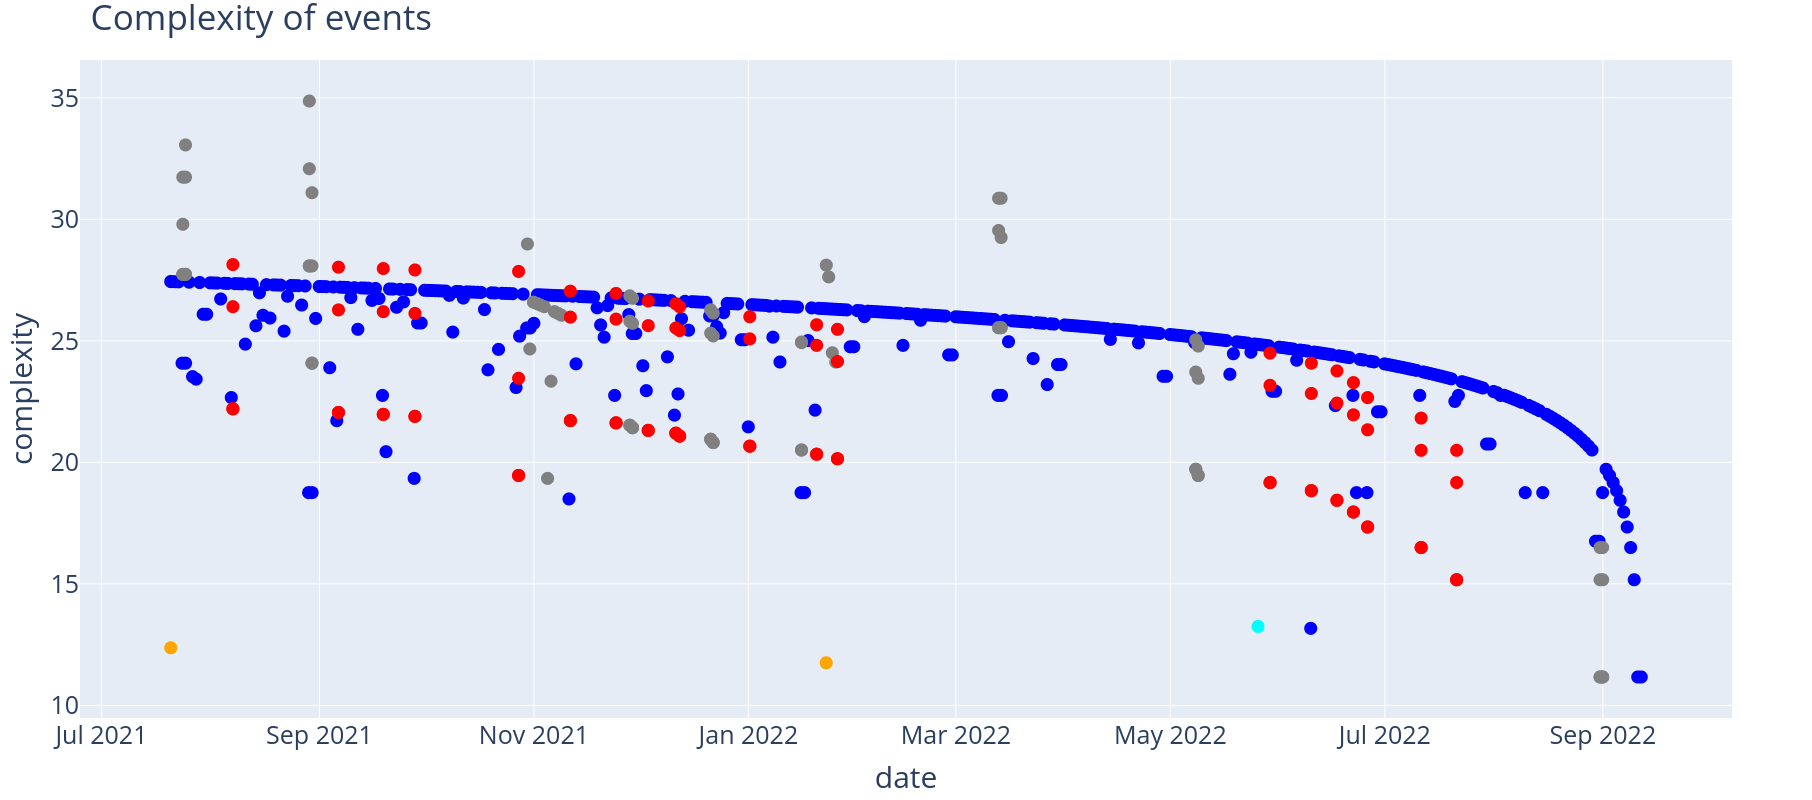
\includegraphics[width=.9\linewidth]{figures/complexity_scenar_2.png}
    \caption{Computed description complexities of events with retrieval paths of
        length at most 4. Events of type ``day'' (blue), ``hot'' (red), ``cold''
        (gray), ``device removal''(orange) and ``device addition'' (cyan) are shown. Events mentioned in the text are specified.}
    \label{fig:computed_cplx}
\end{figure}

The ``memorability score'' is shown in Figure \ref{fig:result1}. Similar to what happened with the description complexity score, most events appear with a low memorability: this corresponds mostly to events from the ``main sequence'' from Figure. \ref{fig:computed_cplx}. On the other hand, some events stand out : for instance events 20 and 329, which are respectively the hottest and coldest days recorded, or event 183 which correspond to the rare type \emph{device\_removal}.
Since our memorability measure treats unusually complex or unusually simple events the
same way (from the absolute value operation in Equation \ref{eq:unexpected}), we
observe that some events are memorable due to their context only. For instance,
the group to which event 149 belongs appears more complex than expected: the same event occurring simultaneously in all four rooms of the house make each instance harder to discern.
Table \ref{tab:paths} illustrates this by exhibiting the retrieval paths used for complexity computation for these events.

\begin{figure}[ht]
    \centering
    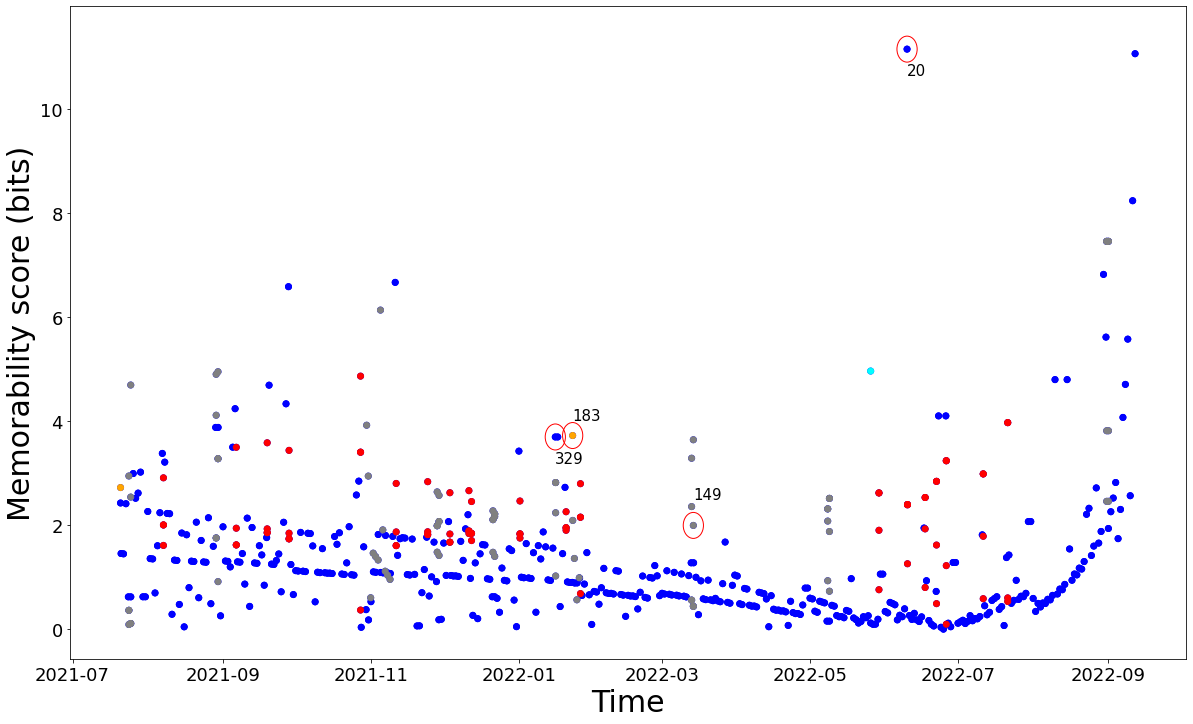
\includegraphics[width=.8\linewidth]{figures/memo_scenar_2.png}
    \caption{Memorability score for events in memory}
    \label{fig:result1}
\end{figure}

\begin{table}
    \centering
    \begin{tabular}{c|c|c}
        Event iD & Event Type    & Retrieval Path                             \\
        \hline
        20       & day           & Label("day"), AxisRank(0, "max\_temp")     \\
        329      & day           & Label("day"), AxisRank(0, "min\_temp")     \\
        183      & deviceRemoval & Label("deviceRemoval"), Day(0)             \\
        149      & cold          & Label("cold"), Day(2), Device("thermo\_2") \\
    \end{tabular}
    \caption{Selected events from the ``temperature example'' with their shortest retrieval path.}
    \label{tab:paths}
\end{table}

Given that we generated the data used for this experiment, it is possible to
flag all perturbation events from the usual daily events and evaluate how a
detection based on ``memorability'' score would perform in distinguishing these
events. The result is presented as a ROC curve in Figure \ref{fig:roc}. This shows the memorability score's performance as a classifying tool for ``out-of-the norm'' events. In this example, memorability alone correctly identified 18 manually generated events with only 5 false-positives. While the direct application of memorability for classification or event detection is not within the scope of this paper (see Section \ref{sec:related} for complexity-based detection), this first result is on par with the motivation of memorability being in accordance with the intuitive notion.

\begin{figure}[ht]
    \centering
    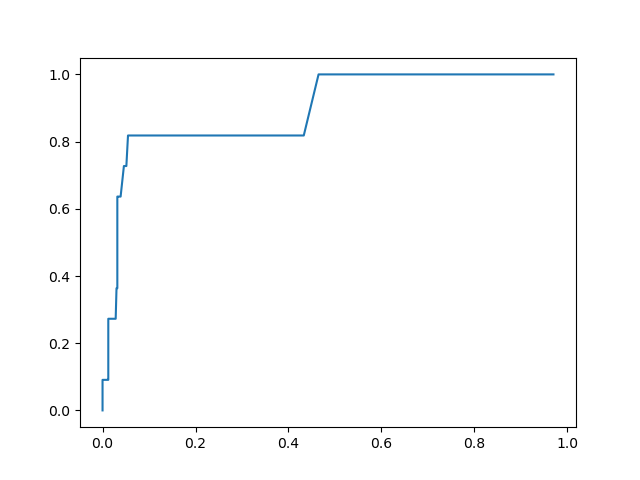
\includegraphics[width=0.7\linewidth]{./figures/roc}
    \caption{Experimental ROC curve (True Positive Rate against False Positive
        Rate) for a classifier based on our memorability score. Measures consider 23
        manually flagged events as memorable (events added to the normal background
        as described in Section~\ref{sec:example}.)}
    \label{fig:roc}
\end{figure}

% \paragraph{Abduction}
% As an illustration of the abductive inference made possible our memorability
% score, we used as a target anomaly the temperature drops visible in the raw
% time series data from our scenario (fig \ref{fig:ts_example}).

% \textbf{TODO: the figure is still missing!}



%%%%%%%%%%%%%%%%%%%%%%%%%%%%%%%%%%%%%%%%%%
\section{Discussion}

\subsection{Related Works}
\label{sec:related}
Our work is intended to be integrated into larger-scale frameworks to monitor
and detect events in complex environment such as smart homes. In these works, the
approach to smart homes is often regarded as self-organizing systems \cite{kramer_rigorous_2009,kounev_notion_2017}. As such, they present capacities of adaptation to new goals,
new components, new environment. A commonly used approach is the principle of
autonomic system, which minimizes user's intervention for management of the
system \cite{kounev_notion_2017,kephart_vision_2003}.

We want to inscribe our work among other classical concurrent approaches to
abduction. In situations where more data is available, we could for instance rely
on correlation or causal inference from known relations \cite{peters_elements_2017,fadiga_or_2021}.
Previous relations between inference and complexity have been studied. In fact, the
case of inference was one of the motivations for R. Solomonoff to introduce his
universal algorithmic probability \cite{solomonoff_formal_1964} as a tool to
reach an idealized inference machine, creating the notion of complexity concomitantly
to Kolmogorov. Subsequently, notions of complexity re-emerged in causal inference:
\cite{janzing_causal_2010} found, when a causal link exists between two random variables,
considering the direct joint probability is simpler, in terms of Kolmogorov complexity,
than the inverse direction.

The relation between complexity, compression and causality was used in \cite{tatti_finding_2008} to devise the PACK algorithm. It models a dataset by using a family of decision trees where each tree describes how one variable can be expressed given the others. By choosing the model minimizing the total description length (i.e. description of the model and description of the errors), PACK compresses the dataset while finding relations between variables which can be further analyzed. More recently, \cite{marx_causal_2018} used Minimum Description Length to determine, given a joint probability distribution over $(X,Y)$, whether $X$ causes $Y$ or $Y$ causes $X$. Their method is based on tree models, and implying that a model respecting the causal relation will be simpler to describe.


Another topic where AIT can provide original approaches is event mining in data streams.
\cite{aggarwal_outlier_2017} provides a good review of modern approaches and techniques
in the field. Some previous work can also be noted for having used AIT techniques to qualify and detect events in time series data. For instance, \cite{batista_complexity-invariant_2011,fadlallah_weighted-permutation_2013} propose weighted permutation entropy as a proxy for complexity measures in time series data, and use it to find relations between different time series. \cite{hu_discovering_2011} proposes a MDL approach to find the intrinsic dimensions of time series. All these approaches are interesting, and can be integrated into our canvas as tools to detect events using only complexity. Using this, one could achieve a purely complexity-driven process for detecting and qualifying events.

The philosophy of our approach can be closely related to the ``Isolation forests'' method\cite{liu_isolation_2008,hariri_extended_2021}. It evaluates the isolation of data points by constructing random binary tree classifiers. On average, outlier points will require less operations to be singled out. Using the average height of leaves in the tree as a metrics, this approach succeeds in identifying outlier points without having to define a ``typical'' point. This approach can be understood in terms of complexity: each node of binary tree classifier needs a fixed amount of information to be described (which variable and threshold are used). So nodes that place higher need less information to be described. As such, outliers need less information to be singled out. Compared to ours, this method is tailored for data-points living in the same metric space. By using predicates as a proxy for complexity computation, our methods is more general, as it is agnostic regarding the nature of events. However, the introduction of predicates adds a subjectivity in the determination of memorable points, as we will discuss later.

While all these works advocate in favor of a strong link between complexity and the
discovery of causes, not other works extends the notion up to the point we propose in this paper, using complexity only as a tool to express the intuitive notion of memorability, and using it for inference.

\subsection{Perspectives}
\label{sec:future}

The practical application of the theoretical notions of memorability and relative memorability requires future developments. In this section, we have selected two of them which seem to us, to date, the most challenging.


First, the main limitation of the current approach is the requirement of
predefined predicate concepts, from which the different filters are constructed.
As an extension, we suggest that in the future, we could explore online
generation of such predicate. A possibility would be to analyze discriminating
dimensions of incoming data and create predicate as to name these differences,
similar to the contrast operations proposed in \cite{dessalles_conceptual_2015,
    gardenfors2004conceptual}. For instance, the predicate concept $\mathtt{hot}$
can be discovered by discriminating a recent hot day along the
temperature axis and naming the difference with the prototypical day.

% ? Maybe a small part on the importance of the introduction of the random pick predicate ?
% The stark difference observed between the two examples in this work shows the importance of being able to select a random event from the set of 

While the execution time is not part of the theoretical view of complexity, it
is of prime importance for practical applications, especially when one considers
implementation into real-time systems or embedded devices. While the computation
we propose appear to be heavy, and possibly heavier as the number of allowed
predicates grows, significant time savings can be achieve by trimming the base
memory of past events deemed the most ``non memorable''. For instance, one can
only retains the 100 most memorable events from the past. The difficulty with
this approach is that such operations should be done in a manner to not
interfere with the complexity computations for new elements: by forgetting some
past events, even uninteresting ones, one should make sure to keep track of what
made the interesting ones, interesting. Investigation of how to do so can pave
the way towards practical implementations and dynamic selection of interesting
events and help reducing the memory and computation cost of data-driven applications.


%%%%%%%%%%%%%%%%%%%%%%%%%%%%%%%%%%%%%%%%%%
\section{Conclusions}
The introduction of description complexity and the subsequent memorability measure allow to compare events of various types with different characteristics. As such, it provides a formal and generic framework to discriminate peculiar events and outliers.

The computation being based on predicates, the memorability score is entirely dependent on their definitions. This can be seen as a caveat or a feature of our approach: it makes the measure subjective while enabling the consideration of user's preferences in the definition and choice of predicates. This consideration can be the topic of future research and open up potential applications.



%%%%%%%%%%%%%%%%%%%%%%%%%%%%%%%%%%%%%%%%%%
\vspace{6pt}

%%%%%%%%%%%%%%%%%%%%%%%%%%%%%%%%%%%%%%%%%%
%% optional
%\supplementary{The following are available online at \linksupplementary{s1}, Figure S1: title, Table S1: title, Video S1: title.}

% Only for the journal Methods and Protocols:
% If you wish to submit a video article, please do so with any other supplementary material.
% \supplementary{The following are available at \linksupplementary{s1}, Figure S1: title, Table S1: title, Video S1: title. A supporting video article is available at doi: link.} 

%%%%%%%%%%%%%%%%%%%%%%%%%%%%%%%%%%%%%%%%%%
\authorcontributions{Conceptualization, É. Houzé and J-L. Dessalles; methodology, software, validation, writing--original draft, É. Houzé; supervision, writing--review and editing J-L. Dessalles, A. Diaconescu and D. Menga. All authors have read and aggreed to the submitted version of the manuscript.
}



\funding{\textbf{TODO je ne sais pas quoi mettre ici ? Indiquer le financement de la thèse ?}}


\dataavailability{All code and data used for the experiments can be found at \url{https://github.com/EtienneHouze/memorability_code}. The iCasa smart home simulator from the Adele research Group, which was used to generate sensor data, can be found at: \url{http://adeleresearchgroup.github.io/iCasa/snapshot/index.html}}

% \acknowledgments{In this section you can acknowledge any support given which is not covered by the author contribution or funding sections. This may include administrative and technical support, or donations in kind (e.g., materials used for experiments).}

\conflictsofinterest{The authors declare no conflict of interest.}

%% Optional
% \sampleavailability{Samples of the compounds ... are available from the authors.}

%%%%%%%%%%%%%%%%%%%%%%%%%%%%%%%%%%%%%%%%%%
%% Only for journal Encyclopedia
%\entrylink{The Link to this entry published on the encyclopedia platform.}

%%%%%%%%%%%%%%%%%%%%%%%%%%%%%%%%%%%%%%%%%%
%% Optional
% \abbreviations{Abbreviations}{
%     The following abbreviations are used in this manuscript:\\

%     \noindent
%     \begin{tabular}{@{}ll}
%         MDPI & Multidisciplinary Digital Publishing Institute \\
%         DOAJ & Directory of open access journals              \\
%         TLA  & Three letter acronym                           \\
%         LD   & Linear dichroism
%     \end{tabular}}

%%%%%%%%%%%%%%%%%%%%%%%%%%%%%%%%%%%%%%%%%%
%% Optional
% \appendixtitles{no} % Leave argument "no" if all appendix headings stay EMPTY (then no dot is printed after "Appendix A"). If the appendix sections contain a heading then change the argument to "yes".
% \appendixstart
% \appendix
% \section{}
% \subsection{}
% The appendix is an optional section that can contain details and data supplemental to the main text---for example, explanations of experimental details that would disrupt the flow of the main text but nonetheless remain crucial to understanding and reproducing the research shown; figures of replicates for experiments of which representative data are shown in the main text can be added here if brief, or as Supplementary Data. Mathematical proofs of results not central to the paper can be added as an appendix.

% \begin{specialtable}[H]
%     \small
%     \caption{This is a table caption. Tables should be placed in the main text near to the first time they are~cited.\label{tab2}}
%     \begin{tabular}{ccc}
%         \toprule
%         \textbf{Title 1} & \textbf{Title 2} & \textbf{Title 3} \\
%         \midrule
%         Entry 1          & Data             & Data             \\
%         Entry 2          & Data             & Data             \\
%         \bottomrule
%     \end{tabular}
% \end{specialtable}

% \section{}
% All appendix sections must be cited in the main text. In the appendices, Figures, Tables, etc. should be labeled, starting with ``A''---e.g., Figure A1, Figure A2, etc.

%%%%%%%%%%%%%%%%%%%%%%%%%%%%%%%%%%%%%%%%%%
\end{paracol}
%%%%%%%%%%%%%%%%%%%%%%%%%%%%%%%%%%%%%%%%%%
% To add notes in main text, please use \endnote{} and un-comment the codes below.
%\begin{adjustwidth}{-5.0cm}{0cm}
%\printendnotes[custom]
%\end{adjustwidth}
%%%%%%%%%%%%%%%%%%%%%%%%%%%%%%%%%%%%%%%%%%
\reftitle{References}

% Please provide either the correct journal abbreviation (e.g. according to the “List of Title Word Abbreviations” http://www.issn.org/services/online-services/access-to-the-ltwa/) or the full name of the journal.
% Citations and References in Supplementary files are permitted provided that they also appear in the reference list here. 

%=====================================
% References, variant A: external bibliography
%=====================================
\externalbibliography{yes}
\bibliography{biblio}

%=====================================
% References, variant B: internal bibliography
%=====================================
% \begin{thebibliography}{999}
%     % Reference 1
%     \bibitem[Author1(year)]{ref-journal}
%     Author~1, T. The title of the cited article. {\em Journal Abbreviation} {\bf 2008}, {\em 10}, 142--149.
%     % Reference 2
%     \bibitem[Author2(year)]{ref-book1}
%     Author~2, L. The title of the cited contribution. In {\em The Book Title}; Editor1, F., Editor2, A., Eds.; Publishing House: City, Country, 2007; pp. 32--58.
%     % Reference 3
%     \bibitem[Author3(year)]{ref-book2}
%     Author 1, A.; Author 2, B. \textit{Book Title}, 3rd ed.; Publisher: Publisher Location, Country, 2008; pp. 154--196.
%     % Reference 4
%     \bibitem[Author4(year)]{ref-unpublish}
%     Author 1, A.B.; Author 2, C. Title of Unpublished Work. \textit{Abbreviated Journal Name} stage of publication (under review; accepted; in~press).
%     % Reference 5
%     \bibitem[Author5(year)]{ref-communication}
%     Author 1, A.B. (University, City, State, Country); Author 2, C. (Institute, City, State, Country). Personal communication, 2012.
%     % Reference 6
%     \bibitem[Author6(year)]{ref-proceeding}
%     Author 1, A.B.; Author 2, C.D.; Author 3, E.F. Title of Presentation. In Title of the Collected Work (if available), Proceedings of the Name of the Conference, Location of Conference, Country, Date of Conference; Editor 1, Editor 2, Eds. (if available); Publisher: City, Country, Year (if available); Abstract Number (optional), Pagination (optional).
%     % Reference 7
%     \bibitem[Author7(year)]{ref-thesis}
%     Author 1, A.B. Title of Thesis. Level of Thesis, Degree-Granting University, Location of University, Date of Completion.
%     % Reference 8
%     \bibitem[Author8(year)]{ref-url}
%     Title of Site. Available online: URL (accessed on Day Month Year).
% \end{thebibliography}

% If authors have biography, please use the format below
%\section*{Short Biography of Authors}
%\bio
%{\raisebox{-0.35cm}{\includegraphics[width=3.5cm,height=5.3cm,clip,keepaspectratio]{Definitions/author1.pdf}}}
%{\textbf{Firstname Lastname} Biography of first author}
%
%\bio
%{\raisebox{-0.35cm}{\includegraphics[width=3.5cm,height=5.3cm,clip,keepaspectratio]{Definitions/author2.jpg}}}
%{\textbf{Firstname Lastname} Biography of second author}

% The following MDPI journals use author-date citation: Admsci,  Arts, Econometrics, Economies, Genealogy, Humanities, IJFS, Jintelligence, JRFM, Languages, Laws, Literature, Religions, Risks, Social Sciences. For those journals, please follow the formatting guidelines on http://www.mdpi.com/authors/references
% To cite two works by the same author: \citeauthor{ref-journal-1a} (\citeyear{ref-journal-1a}, \citeyear{ref-journal-1b}). This produces: Whittaker (1967, 1975)
% To cite two works by the same author with specific pages: \citeauthor{ref-journal-3a} (\citeyear{ref-journal-3a}, p. 328; \citeyear{ref-journal-3b}, p.475). This produces: Wong (1999, p. 328; 2000, p. 475)

%%%%%%%%%%%%%%%%%%%%%%%%%%%%%%%%%%%%%%%%%%
%% for journal Sci
%\reviewreports{\\
%Reviewer 1 comments and authors’ response\\
%Reviewer 2 comments and authors’ response\\
%Reviewer 3 comments and authors’ response
%}
%%%%%%%%%%%%%%%%%%%%%%%%%%%%%%%%%%%%%%%%%%
\end{document}

